
\subsection{Linux图形系统体系栈}
\subsubsection{早期Linux下的2D图形体系栈}
在早期,Linux下的应用程序的绘制都不是直接绘制,而是通过X-Server来进行绘制。应用程序通过Xlib库并遵守X11协议向X-Server发送渲染指令,然后X-Server接受这些指令并处理和转化为硬件指令,并将这些硬件指令发送给GPU让其执行\cite{Get-X-Off}。具体流程如图\ref{fig:2D-Graph-Stack}所示

\begin{figure}[H] 
  \centering
  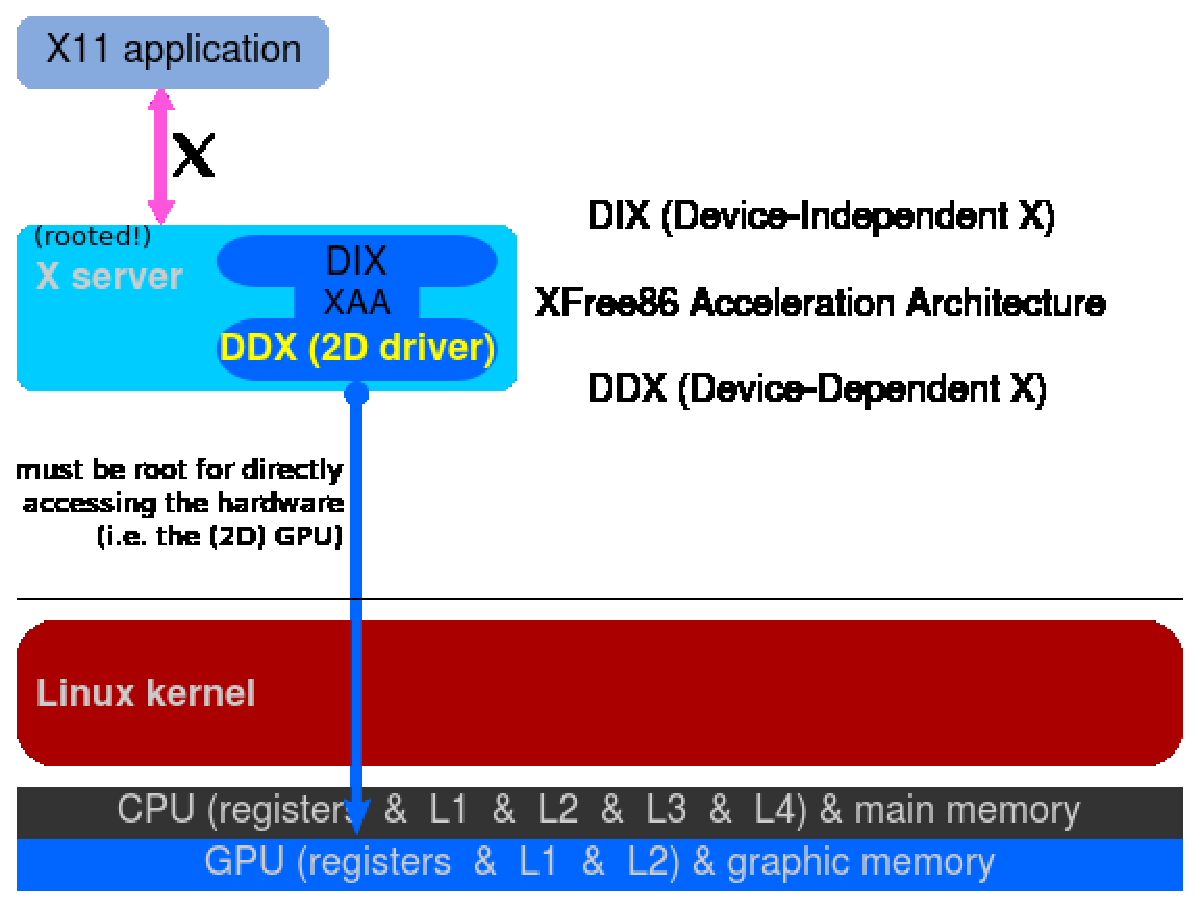
\includegraphics[width=10cm,height=7cm]{figures/chap01/Linux_graphics_drivers_2D}
  \caption{早期Linux下2D图形系统体系栈}
  \label{fig:2D-Graph-Stack}
\end{figure}

\subsubsection{支持3D图形渲染的Linux图形体系栈}
经过不断的发展,Linux通过OpenGL实现了3D图形渲染,其中3D图形渲染的方法主要有两种:
\begin{itemize}
\item{\textbf{Indirect Rendering}}: \\
在一些传统的系统平台上,由于只能唯一通过X-Server访问图形硬件,所以只能向X-Server发送绘制指令然后再通过X-Server转化为硬件命令给GPU执行,这种方式和传统的2D绘制方式相似。
\item{\textbf{Direct Rendering}}: \\ 
随着系统平台上的发展,直接渲染框架(Direct Rendering Infrastructure)的诞生使得OpenGL程序可以通过Linux内核的drm库直接与图形硬件(GPU)进行交互,这一进步极大的提高了3D渲染的效率,成为当今比较主流的渲染方式\cite{Fair-Share}。
\end{itemize}

\begin{figure}[H] 
  \centering
  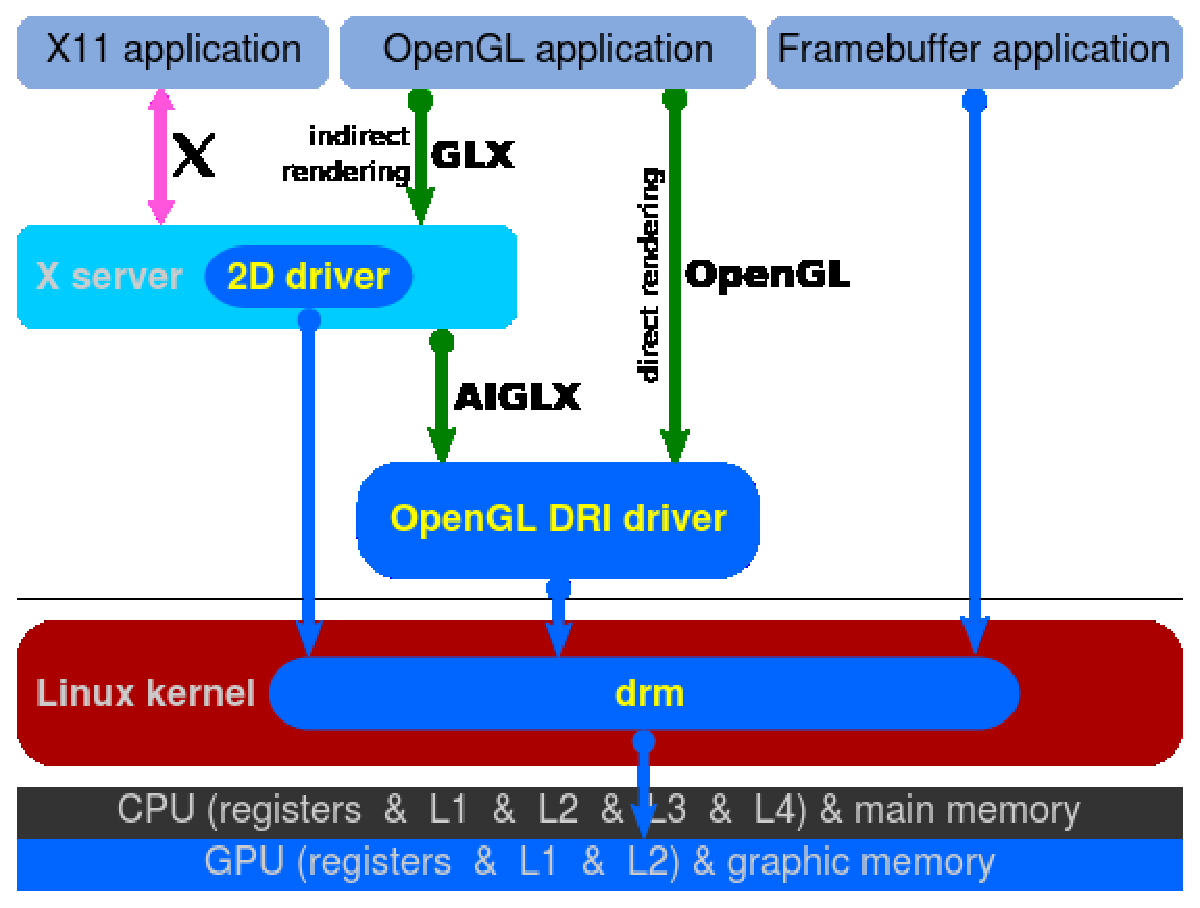
\includegraphics[width=10cm,height=6cm]{figures/chap01/OpenGL_With_Direct_Rendering}
  \caption{Linux下3D图形系统体系栈}
  \label{fig:OpenGL_With_Direct_Rendering}
\end{figure}

\subsubsection{DRM}
DRM(直接渲染管理)是Linux内核的一个负责与GPU通信的子系统,它公开了一套API使得用户空间的程序可以使用它发送命令和数据给GPU,并执行一些诸如配置显示模式的操作\cite{Linux-DRM}。例如,用户空间程序可以使用DRM的API向命令GPU进行硬件加速3D渲染,视频解码以及GPGPU计算。

在DRM被构建出来之前,用户空间的程序只能唯一的直接访问和操作GPU硬件资源(X server),这是因为如果允许两个或者多个用户空间程序同时直接使用GPU资源就会彼此发生冲突而彼此都不能正确的执行(如图\ref{fig:without-drm})。

\begin{figure}[H] 
  \begin{minipage}[t]{0.5\linewidth}
  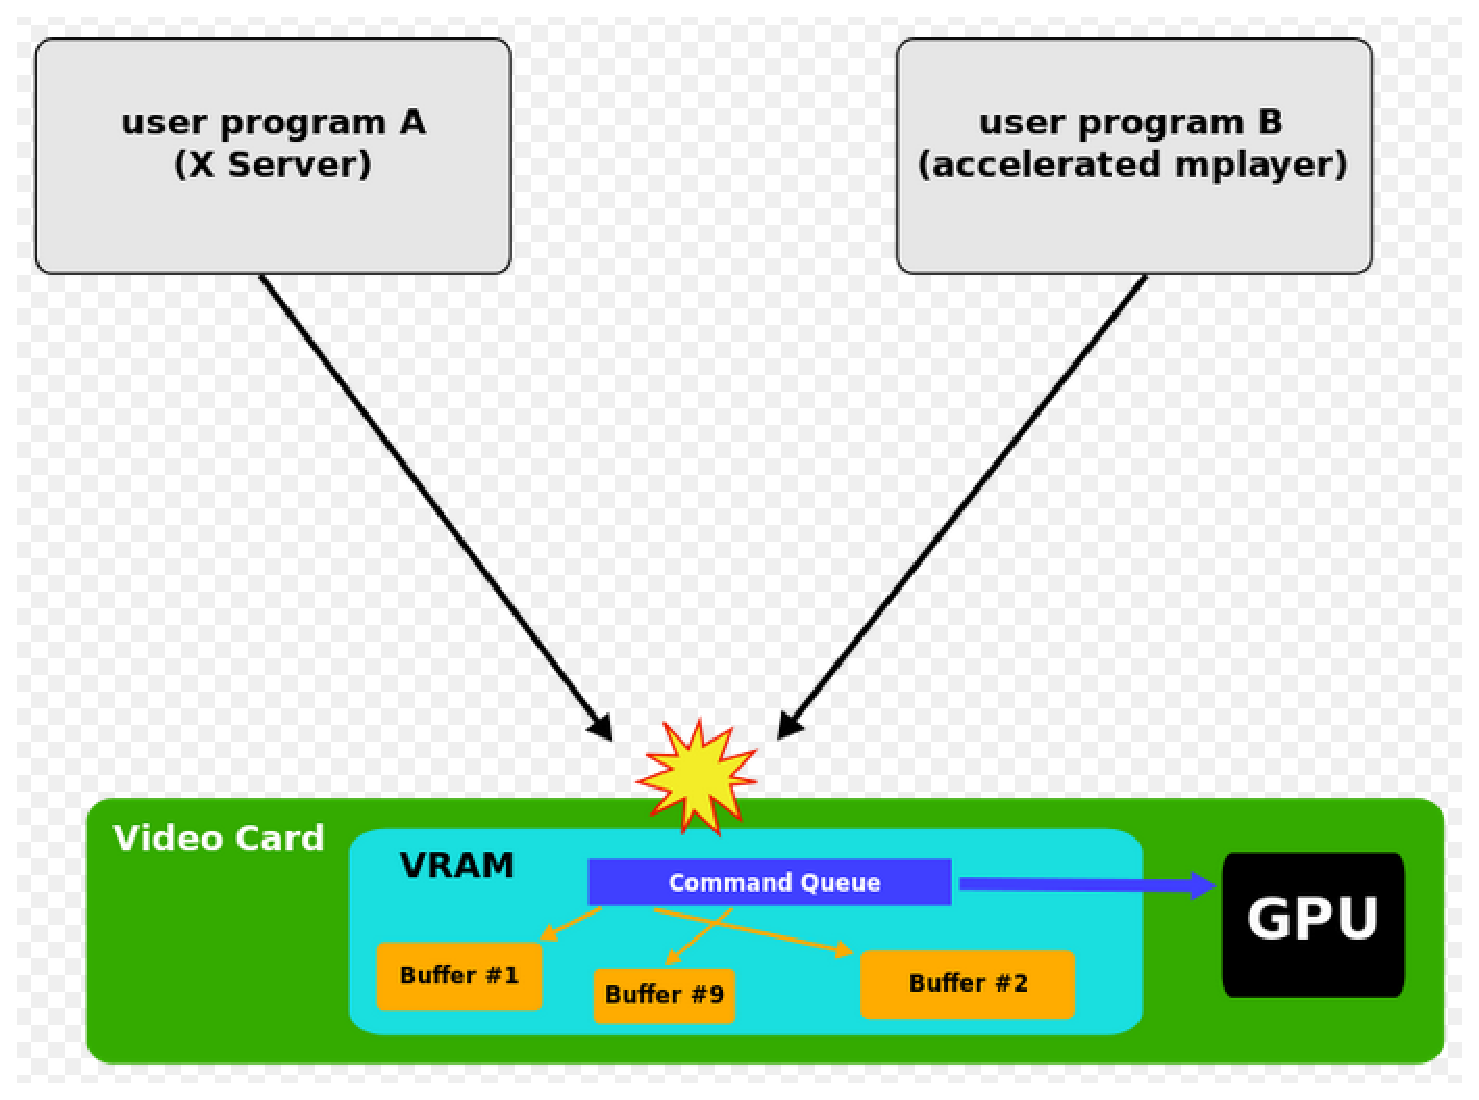
\includegraphics[width=8cm,height=7cm,center]{figures/chap01/without-drm}
  \caption{Without DRM}
  \label{fig:without-drm}
  \end{minipage}
  \begin{minipage}[t]{0.5\linewidth}
  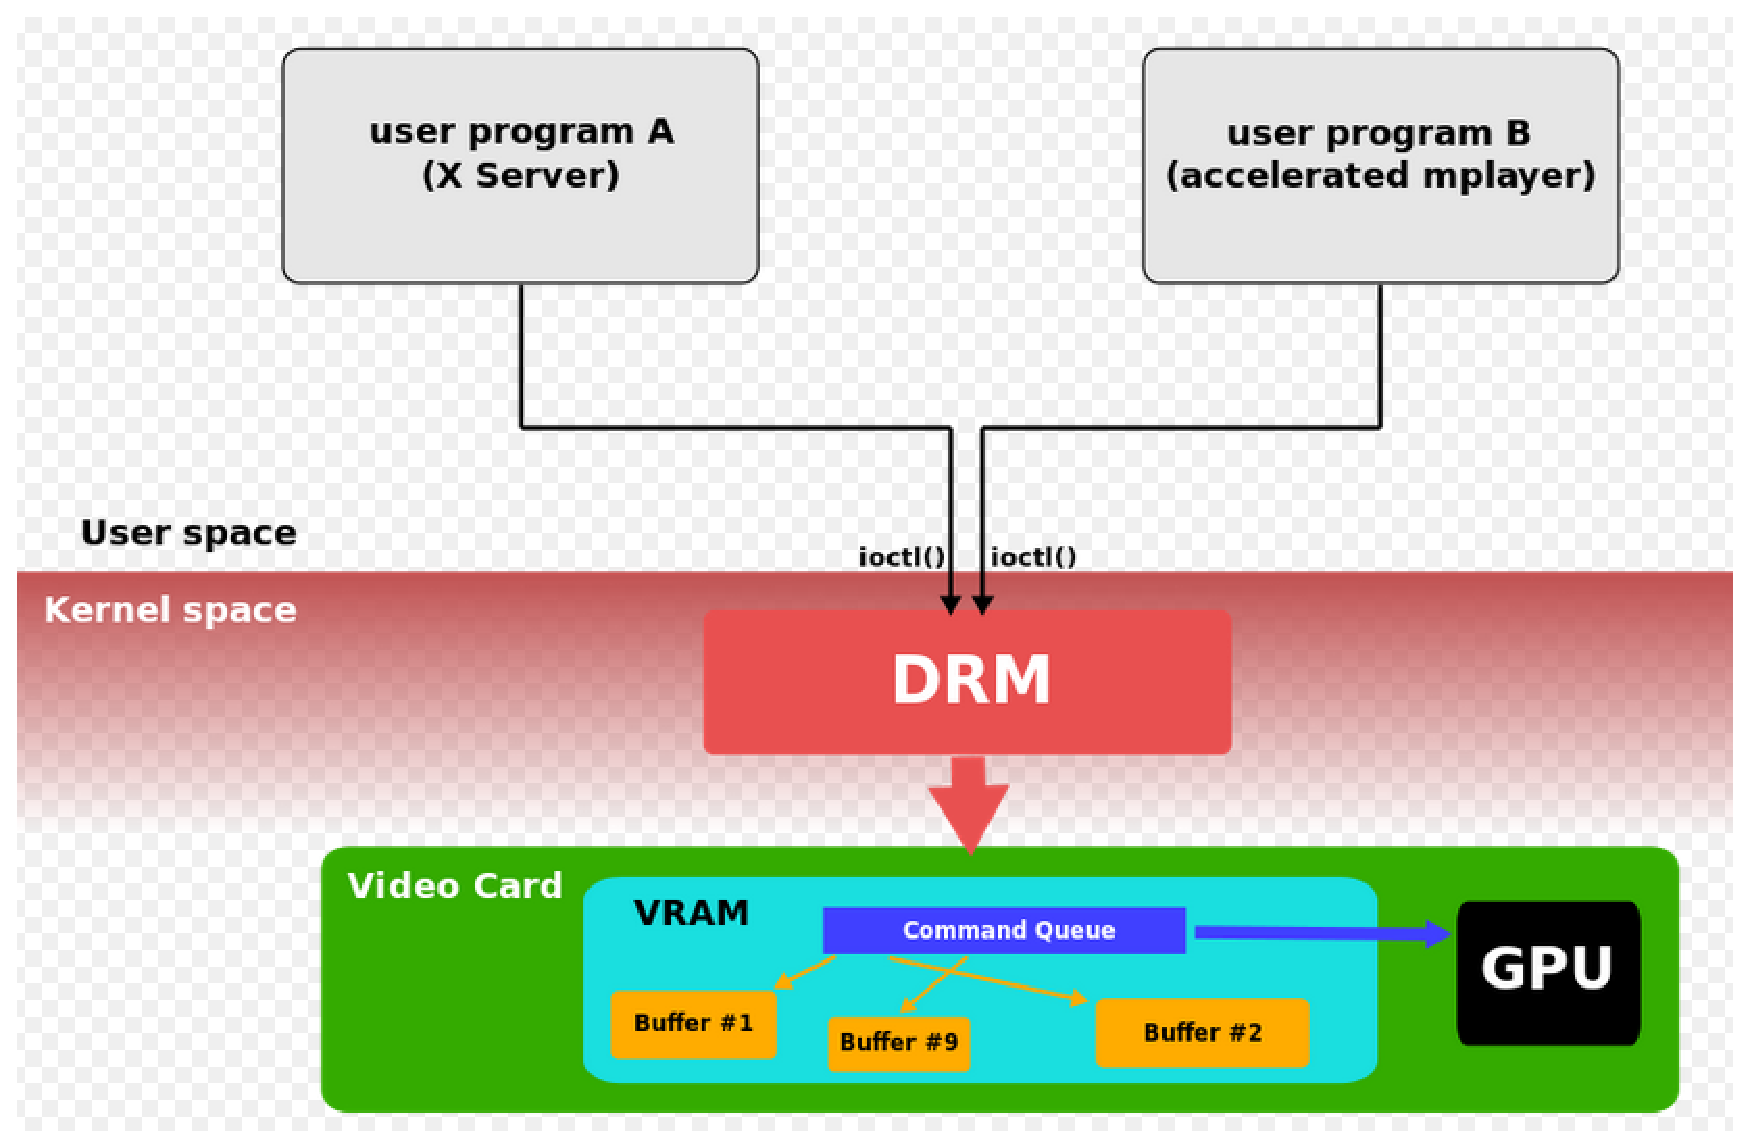
\includegraphics[width=8cm,height=7cm,center]{figures/chap01/with-drm}
  \caption{With DRM}
  \label{fig:with-drm}
  \end{minipage}
\end{figure}

于是,为了能让多个用户空间程序可以共同有效的使用GPU硬件资源,DRM就被发展起来了,它负责初始化和管理命令队列,VRAM以及其他硬件资源,用户空间程序通过请求DRM来实现对GPU硬件资源的共同使用(如图\ref{fig:with-drm})。

\subsection{OpenGL}

\subsubsection{OpenGL基本介绍}
开放图形库(Open Graphics Library,缩写为OpenGL)是个定义了一个跨编程语言、跨平台的应用程序接口(API)的规范,它用于生成2D、3D图像\cite{SuperBible}。这个接口由近350个不同的函数调用组成,用来从简单的图形比特绘制复杂的三维景象。而另一种程序接口系统是仅用于Microsoft Windows上的Direct3D。OpenGL常用于CAD、虚拟实境、科学可视化程序和电子游戏开发。

OpenGL规范描述了绘制2D和3D图形的抽象API。尽管这些API可以完全通过软件实现,但它是为大部分或者全部使用硬件加速而设计的。OpenGL不仅语言无关,而且平台无关。规范只字未提获得和管理OpenGL上下文相关的内容,而是将这些作为细节交给底层的窗口系统。出于同样的原因,OpenGL纯粹专注于渲染,而不提供输入、音频以及窗口相关的API\cite{OpenGL-Wiki}。

\subsubsection{OpenGL渲染管线}

绝大多数OpenGL实现都有着相似的操作,一系列相关的处理阶段叫做OpenGL渲染管线。图\ref{fig:OpenGL-Pipeline}显示了这些顺序,几何数据(顶点、直线和多边形)所经历的处理阶段包括求值器和基于顶点的操作,而像素数据(像素、图像和位图)的处理过程则有所不同。在最终的像素数据写入到帧缓存之前,这两种类型的数据都经过相同的最终步骤(光栅化和基于片段的操作)\cite{OpenGL-Programming-Guide}。

\begin{figure}[H] 
  \centering
  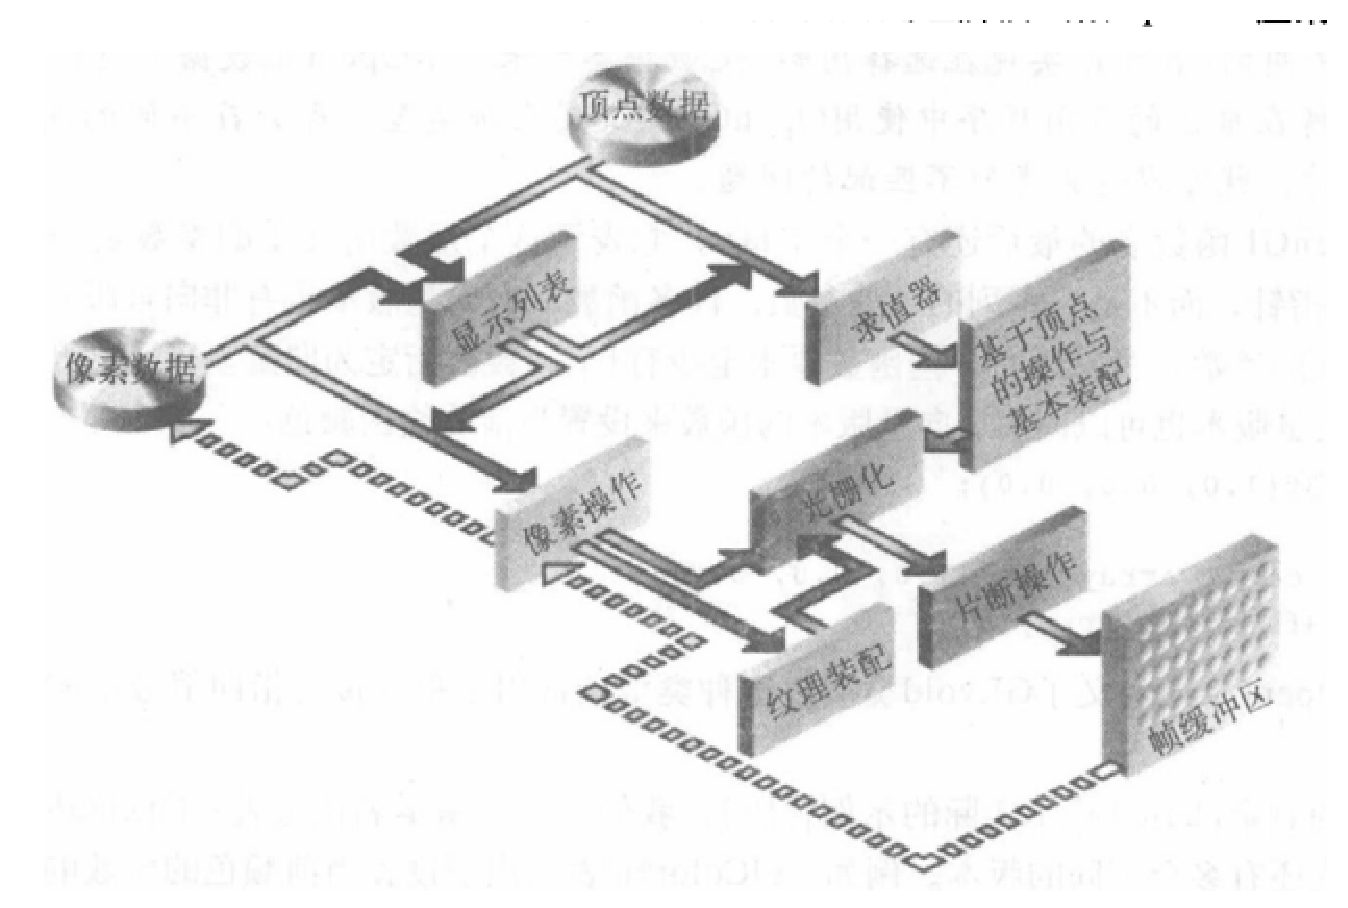
\includegraphics[width=10cm,height=7cm]{figures/chap01/OpenGL-Pipeline}
  \caption{OpenGL渲染管线}
  \label{fig:OpenGL-Pipeline}
\end{figure}

这里详细介绍一下渲染管线上的几个阶段:
\begin{itemize}
\item{\textbf{显示列表}}:\quad几何图形和像素都可以保存到显示列表中,以供当前或者以后使用。当一个显示列表被执行时候,保存的数据就从显示列表取出,就像在立即模式下直接由应用程序发送的那样。
\item{\textbf{求值器}}:\quad所有的几何图形都最终要通过顶点来表示。求值器提供了一种方法,它根据曲线或者表面的控制顶点计算表示曲线或者表面的顶点。这种方法是一种多项式映射,它可以根据控制点产生表面法线,纹理坐标等。
\item{\textbf{基于顶点的操作与图元装配}}:\quad这其实是两个过程,首先基于顶点的操作是把顶点转化为图元,即将空间坐标从3D世界的一个位置投影到屏幕的一个位置。其次图元装配阶段主要内容就是裁剪,它的任务是消除位于某个特定平面以外的部分几何图元。
\item{\textbf{像素操作}}:\quad通常需要对来自系统内存的一个数组中的像素进行解包,接着这些像素数据会被执行像素转化(缩放、偏移、映射和截取)操作。
\item{\textbf{纹理装配}}:\quad OpenGL应用程序可以在几何物体上应用纹理图像,此阶段就是纹理相关的装配处理。
\item{\textbf{光栅化}}:\quad把几何数据和像素数据转化为片段的过程。每个片段对应于帧缓存的一个像素。这个过程会考虑直线的宽度,点的大小,着色模型以及抗锯齿等计算。
\item{\textbf{片段操作}}:\quad数据实际存储到帧缓存区前,还需要执行的一系列操作,比如可能的纹理操作,前面纹理装配阶段产生的纹理内存会为每个片段生成一个纹理单元并与该片段融合。
\end{itemize}

\subsubsection{OpenGL版本变化}
OpenGL是一个不断进化的API。新版OpenGL规范会定期由Khronos Group发布,新版本通过扩展API来支持各种新功能。每个版本的细节由Khronos Group的成员一致决定,包括显卡厂商、操作系统设计人员以及类似Mozilla和谷歌的一般性技术公司。详细历史版本更新参阅附录\ref{cha:OpenGL-History-Version}。

